\subsection[Grenzen der Diagonalisierung]{Grenzen der Diagonalisierung}
\begin{frame}
	\frametitle{Grenzen der Diagonalisierung}
	\framesubtitle{Wiederholung Diagonalisierung}
	\begin{KITinfoblock}{Was ist Diagonalisierung} {
			Als Diagonalisierung wird (hier) ein Beweis bezeichnet, der nur auf den beiden folgenden
			Eigenschaften von TM aufbaut.
			
			\begin{enumerate}
				\item<2-> Die Existenz einer Repräsentation von TM durch Zeichenketten (Gödelnummer)
				\item<3-> Die Fähigkeit eine andere TM mit geringem zusätzlichen Zeit- oder Platzbedarf zu simulieren (Universelle TM)
			\end{enumerate}		
		}
	\end{KITinfoblock}
\end{frame}

\begin{frame}
	\frametitle{Grenzen der Diagonalisierung}
	\framesubtitle{Definition von Orakelmschinen}
	\begin{KITinfoblock}{Definition Orakel-Turingmaschine} {
			Eine Orakel-Turingmaschine $M$ ist eine TM, die folgende zusätzliche Eigenschaften hat:
			\begin{itemize}
				\item<2-> ein spezielles zusätzliches Band (Orakelband) und 3 spezielle zusätzliche Zustände $q_{query}, q_{yes}, q_{no}$.
				\item <3-> ein Orakel $O \subset \{0,1\}^*$
				\item <4-> Wenn $M$ den Zustand $q_{query}$ betritt, ist der Folgezustand
					\begin{itemize}
					\item $q_{yes}$, wenn für Inhalt $s$ des Orakelbands gilt $s \in O$ und
				    \item	$q_{no}$, wenn  $s \notin O$ 
					\end{itemize} 
				\item<5-> Das Orakel liefert die Antwort \alert{in einem Berechnungsschritt}
			\end{itemize}
		}
	\end{KITinfoblock}
\end{frame}
\begin{frame}
	\frametitle{Grenzen der Diagonalisierung}
	\framesubtitle{Satz von Baker-Gill-Solovay}
	\begin{KITinfoblock}{Satz (Baker,Gill,Solovay, 75)}
		Es existieren Orakel A, B so dass ${\P}^A = {\NP}^A$ und ${\P}^B \neq {\NP}^B$
	\end{KITinfoblock}
	\bigskip
	\pause
	\begin{overprint}
		\only<2-3>{
		
		\begin{KITinfoblock}{relativierende Beweise}
			Wir nennen einen Beweis, der auch für TM mit Orakel gilt, einen \newline
			\emph{relativierenden Beweis}
		\end{KITinfoblock}
		\begin{itemize}[<+->]
		\item Diagonalisierung ist relativierend und kann damit nicht f\"ur die $\P
		- \NP$ Frage genutzt werden.
		\item $\Rightarrow$ ein Beweis für die $\P-\NP$ Frage muss ein nicht
		relativierendes Verfahren nutzen !
		\end{itemize}
		}
		
	\end{overprint}
\end{frame}

\begin{frame}
	\frametitle{Grenzen der Diagonalisierung}
	\framesubtitle{Beweis : ${\P}^A = {\NP}^A$ }
	\begin{itemize}[<+->]
	
	\item ${\P}^A = {\NP}^A$ haben wir gerade schon gesehen:
			Nutze einfach das Orakel A = $\mathbf{EXPCOM}$
	\item B zu konstruieren ist schwieriger (und interessanter!)
	\end{itemize}	
\end{frame}

\begin{frame}
	\frametitle{Grenzen der Diagonalisierung}
	\framesubtitle{Beweis : ${\P}^B \neq {\NP}^B$}
	\begin{KITinfoblock}{Definition unäre Sprache $U_B$}
		Für eine Sprache B sei $U_B = \lbrace 1^n :$ Es gibt einen String
		der L\"ange n in B $\rbrace $
	\end{KITinfoblock}	
	\pause
	
	\begin{itemize}[<+->]
		\item Wir sehen sofort ein : $U_B \in {\NP}^B$ , da eine nicht det. TM
			ein Zertifikat raten kann.
		\item M\"ussen also nur noch B so konstruieren, dass $U_B \notin {\P}^B$
	\end{itemize}
\end{frame}

\begin{frame}
	\frametitle{Grenzen der Diagonalisierung}
	\framesubtitle{Konstruktion von B}
	Wir konstruieren eine Folge von Sprachen $(B_i)_{i \in \mathbb{N}}$ so , dass 
	$B = \lim_{n \to \infty} B_i$	
	\begin{itemize}[<+->]
		\item Wie stellen wir sicher, dass alle Turing Maschinen $U_B$ nicht
			in polynomieller Zeit entscheiden können?
		\item Tipp: Die Menge aller Turing Maschinen ist abzählbar
	\end{itemize}
\end{frame}

\begin{frame}
	\frametitle{Grenzen der Diagonalisierung}
	\framesubtitle{Konstruktion von B}
	\begin{itemize}[<+->]
	\item Genau : Wir iterieren über alle Turing Maschinen $M_i$ und stellen
	sicher, dass $M_i$ nicht in polynomieller Zeit $U_B$ entscheiden kann
	\item Nutze dabei, dass die Anzahl der Wörter exponentiell in der Eingabelänge wächst
	\end{itemize}
\end{frame}

\begin{frame}
	\frametitle{Grenzen der Diagonalisierung}
	\framesubtitle{Konstruktion von B}
	Wir fangen an mit $B_0 = \emptyset$. Konstruktion f\"r $B_i$ :
	\begin{itemize}
		\item Wähle n so , dass n größer als alle Strings in $B_{i-1}$
		\item Lasse $M_i$ auf Eingabe $1^n$ genau $2^n / 10$ Schritte laufen \newline
			(Beachte, dass $M_i$ das Orakel B hat!)
		\item 
	\end{itemize}
\end{frame}
\begin{frame}
	\frametitle{Grenzen der Diagonalisierung}
	\framesubtitle{Konstruktion von B}
	\begin{columns}
	\column{.5\textwidth}
	
	\only<1>{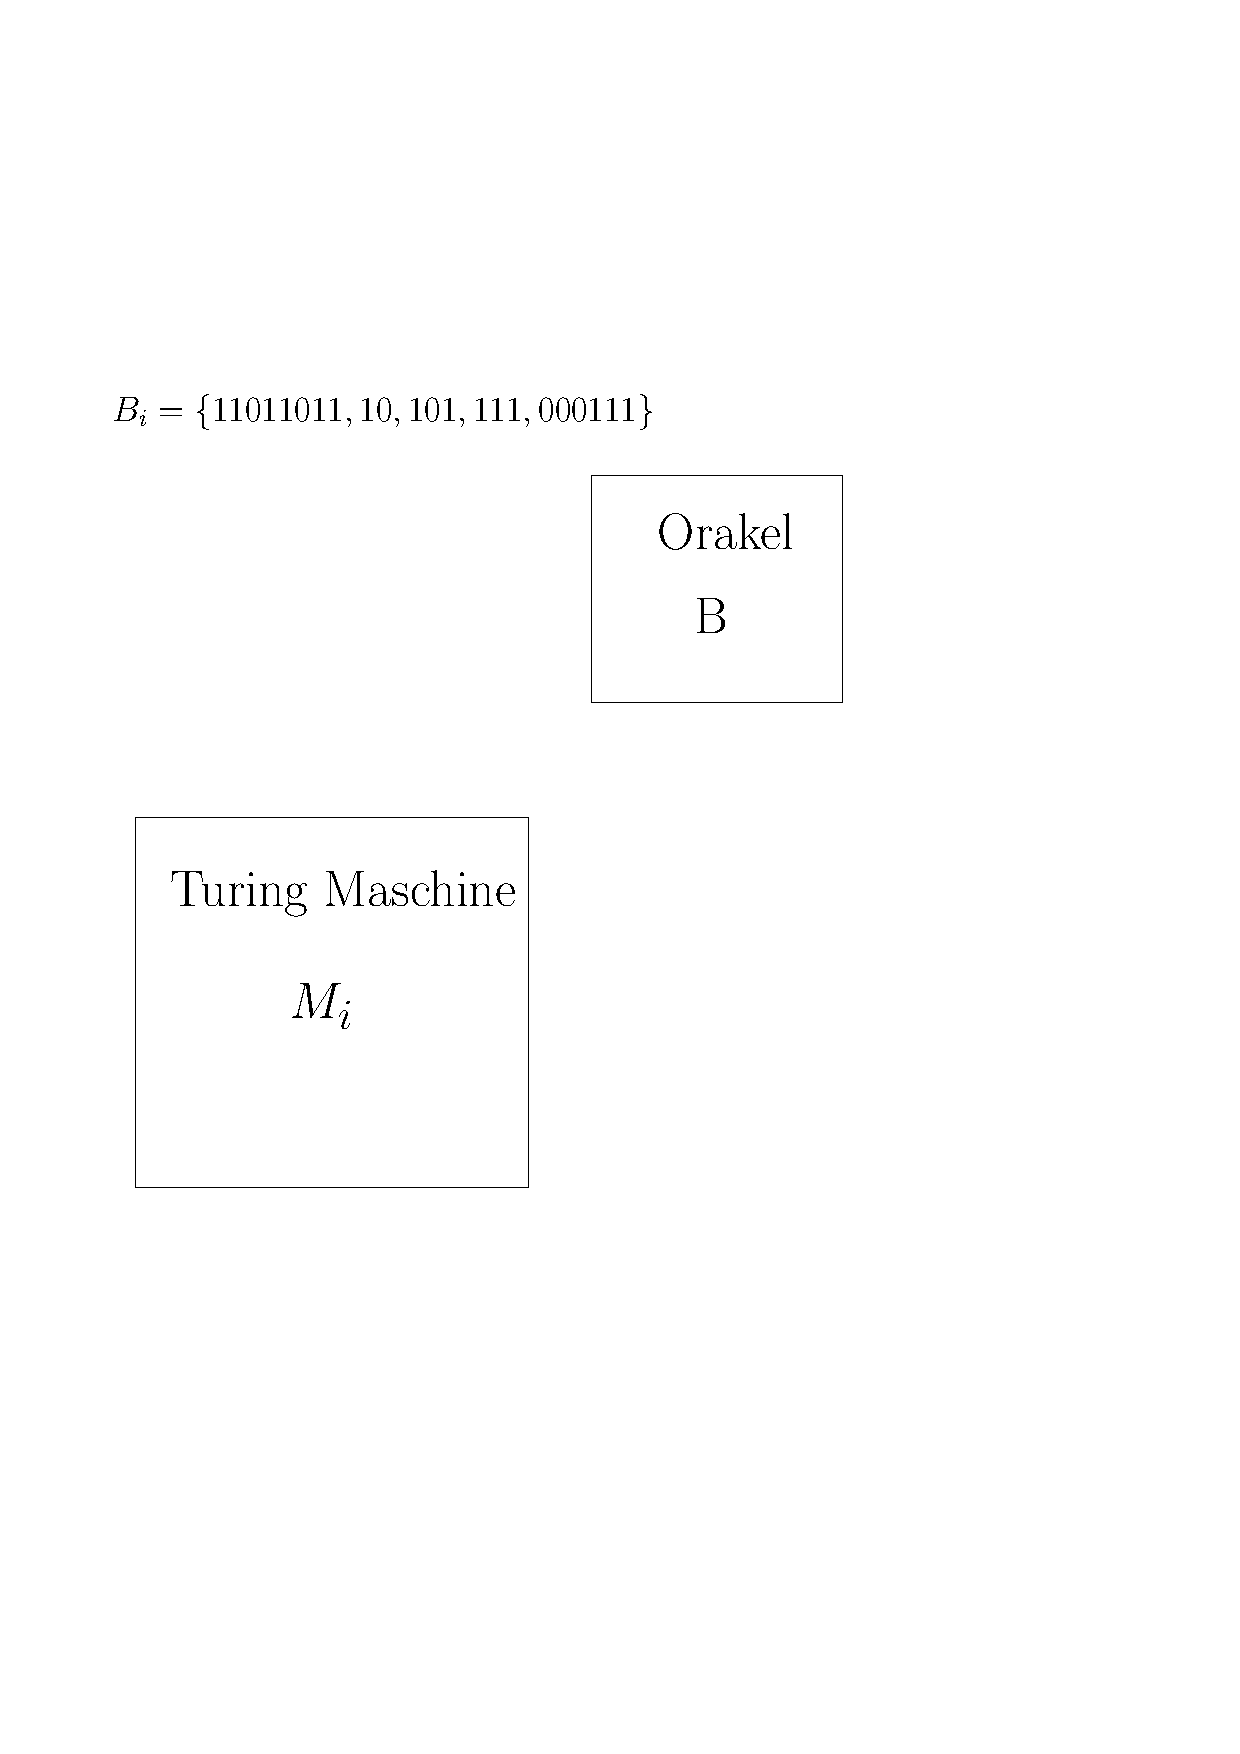
\includegraphics[page=1, scale= 0.5]{images/b_construction.pdf}}
	\only<2>{\includegraphics[page=2, scale= 0.5]{images/b_construction.pdf}}
	\only<3>{\includegraphics[page=3, scale= 0.5]{images/b_construction.pdf}}
	\only<4>{\includegraphics[page=4, scale= 0.5]{images/b_construction.pdf}}
	\only<5>{\includegraphics[page=5, scale= 0.5]{images/b_construction.pdf}}
	\only<6>{\includegraphics[page=6, scale= 0.5]{images/b_construction.pdf}}
	
	\column{.5\textwidth}
	\begin{itemize}
	  \item Das Orakel antwortet konsistent auf dem bisherigen $B_i$
	  \item Wir merken uns alle Strings der L\"ange n, die $M_i$ an fragt!
	\end{itemize}
	\end{columns}
\end{frame}

\begin{frame}
	\frametitle{Grenzen der Diagonalisierung}
	\framesubtitle{Konstruktion von B}
	\begin{itemize}[<+->]
	  \item Wir definieren nun $B_{i+1}$ wie folgt :
	  \item Wenn $M_i$ nicht gehalten hat : $B_{i+1} = B_i$
	  \item ansonsten : \begin{itemize}
	    \item $M_i$ akzeptiert $1^n$ : Wir definieren, dass kein String der Länge n
	    in B ist.
	    \item $M_i$ lehnt ab : Wähle $x \in {\lbrace 0,1 \rbrace}^n$, welches nicht
	    von $M_i$ an gefragt wurde und setze $B_{i+1} = B_i \cup \lbrace x \rbrace$
	    \item warum existiert dieses x?
	    \end{itemize}
	\end{itemize}
\end{frame}

\begin{frame}
	\frametitle{Grenzen der Diagonalisierung}
	\framesubtitle{Beweis Schluss}
	
	\begin{itemize}[<+->]
	  \item Haben oben ein gesehen, dass $U_B \in {\NP}^B$
	  \item Und f\"ur jede polynomiell beschränkte TM M existiert ein i,so dass 
	  	\begin{itemize}
	  	  \item M = $M_i$
	  	  \item M auf der Eingabe $1^i$ weniger als $2^i / 10 $ Schritte benötigt
	  	  \item und damit $M_i$ nach Konstruktion die Frage $1^i \in U_B$ falsch
	  	  beantwortet
	  	 \end{itemize}
	  	\item $\Rightarrow U_B \notin {\P}^B$ und damit ${P}^B \neq {\NP}^B$ \qed
	\end{itemize}
\end{frame}